\documentclass[aspectratio=169]{beamer}
%[handout]

\usetheme[progressbar=frametitle]{metropolis}
\usepackage{appendixnumberbeamer}

\usepackage[utf8]{inputenc}
\usepackage[T1]{fontenc}

\usepackage[brazil]{babel}
\usepackage[outputdir=..]{minted}
\usepackage{xcolor}
\usepackage{soul} % strikethrough
\usepackage{advdate}
\usepackage{graphicx}
\graphicspath{{figs/}}
\usepackage{graphbox}

\usepackage[ampersand]{easylist}

\usepackage{multirow}
\usepackage{multicol}
\usepackage{subcaption}

\usepackage{pgf,tikz}
\usetikzlibrary{shapes,arrows,positioning}
\usetikzlibrary{circuits.logic.US}
\usetikzlibrary{matrix,calc}

\usepackage{karnaugh-map}

\usepackage{pgfpages}
\setbeameroption{hide notes} % Only slides
% \setbeameroption{show only notes} % Only notes
% \setbeameroption{show notes on second screen=right} % Both

% \graphicspath{{../figs/}}

\definecolor{bgc}{rgb}{0.95,0.9,0.95}
\definecolor{links}{HTML}{2A7F7F}
\hypersetup{colorlinks,linkcolor=,urlcolor=links}

\newminted{verilog}{fontsize=\scriptsize, 
    linenos,
    numbersep=8pt,
    bgcolor=bgc,
    tabsize=4,
    framesep=3mm} 
    %frame=lines,

\newcommand{\verilog}[1]{\verilogf{#1}{\footnotesize}}

\newcommand{\verilogf}[2]{\inputminted[fontsize=#2, 
    linenos,
    tabsize=2,
    numbersep=4pt,
    bgcolor=bgc,
    framesep=3mm]{verilog}{../codes/#1.v}
}

\newminted{nasm}{fontsize=\scriptsize, 
		   linenos,
		   numbersep=8pt,
           bgcolor=bgc,
		   framesep=3mm} 

\usepackage{booktabs}
\usepackage[scale=2]{ccicons}

\usepackage{pgfplots}
\usepgfplotslibrary{dateplot}

\usepackage{hyperref}


\usepackage{xspace}
\newcommand{\themename}{\textbf{\textsc{metropolis}}\xspace}



\usepackage{pifont}% http://ctan.org/pkg/pifont
\newcommand{\cmark}{\ding{51}}%
\newcommand{\xmark}{\ding{55}}%

% \tiny	
% \scriptsize
% \footnotesize
% \small	
% \normalsize	
% \large	
% \Large	
% \LARGE	
% \huge	
% \Huge	



\newminted{python}{fontsize=\scriptsize, 
		   linenos,
		   breaklines,
		   numbersep=8pt,
           tabsize=2,
		   framesep=3mm} 
		   
\newminted{verilog}{fontsize=\scriptsize, 
		   linenos,
		   breaklines,
		   numbersep=8pt,
           tabsize=2,
		   framesep=3mm} 
		   




\definecolor{bgc}{rgb}{0.95,0.9,0.95}
\definecolor{links}{HTML}{2A7F7F}
\hypersetup{colorlinks,linkcolor=,urlcolor=links}


% \usepackage[style=apa]{biblatex}
% \addbibresource{mm.bib}


% \author{\large Prof. Ricardo Menotti (\href{mailto:menotti@ufscar.br}{menotti@ufscar.br})}

\newcommand{\newauthor}[2]{
  \parbox{0.50\textwidth}{
    \texorpdfstring
      {
        \centering
        \small #1 \newline
        {\scriptsize{\urlstyle{same}\href{mailto:#2}{#2}\urlstyle{tt}}}
      }
      {#1} \newline
  }
}

\author{
  \newauthor{Prof. Ricardo Menotti}{menotti@ufscar.br}
\and \newauthor{Prof. Luciano de Oliveira Neris}{lneris@ufscar.br}  
%\and \newauthor{Prof. Artino Quintino da Silva Filho}{artino@ufscar.br}
% \and \newauthor{Prof. Maurício Figueiredo}{mauricio@ufscar.br}
% \and \newauthor{Prof. Edilson Kato}{kato@ufscar.br}
% \and \newauthor{Prof. Roberto Inoue}{rsinoue@ufscar.br}
}

\date{Atualizado em: \today}

\institute{\large \textbf{Departamento de Computação} \\
Centro de Ciências Exatas e de Tecnologia \\
Universidade Federal de São Carlos}

\title{Lógica Digital (1001351)}

\titlegraphic{\hfill
\includegraphics[height=1.5cm]{LogoUfscar}}



\subtitle{Circuitos Combinacionais: Conversores de códigos} % 

\begin{document}

\begin{frame}
	\titlepage
\end{frame} 

\section{Decodificadores}

\begin{frame}{\insertsection}   \centering
    \begin{columns}
        \begin{column}{0.40\textwidth}
        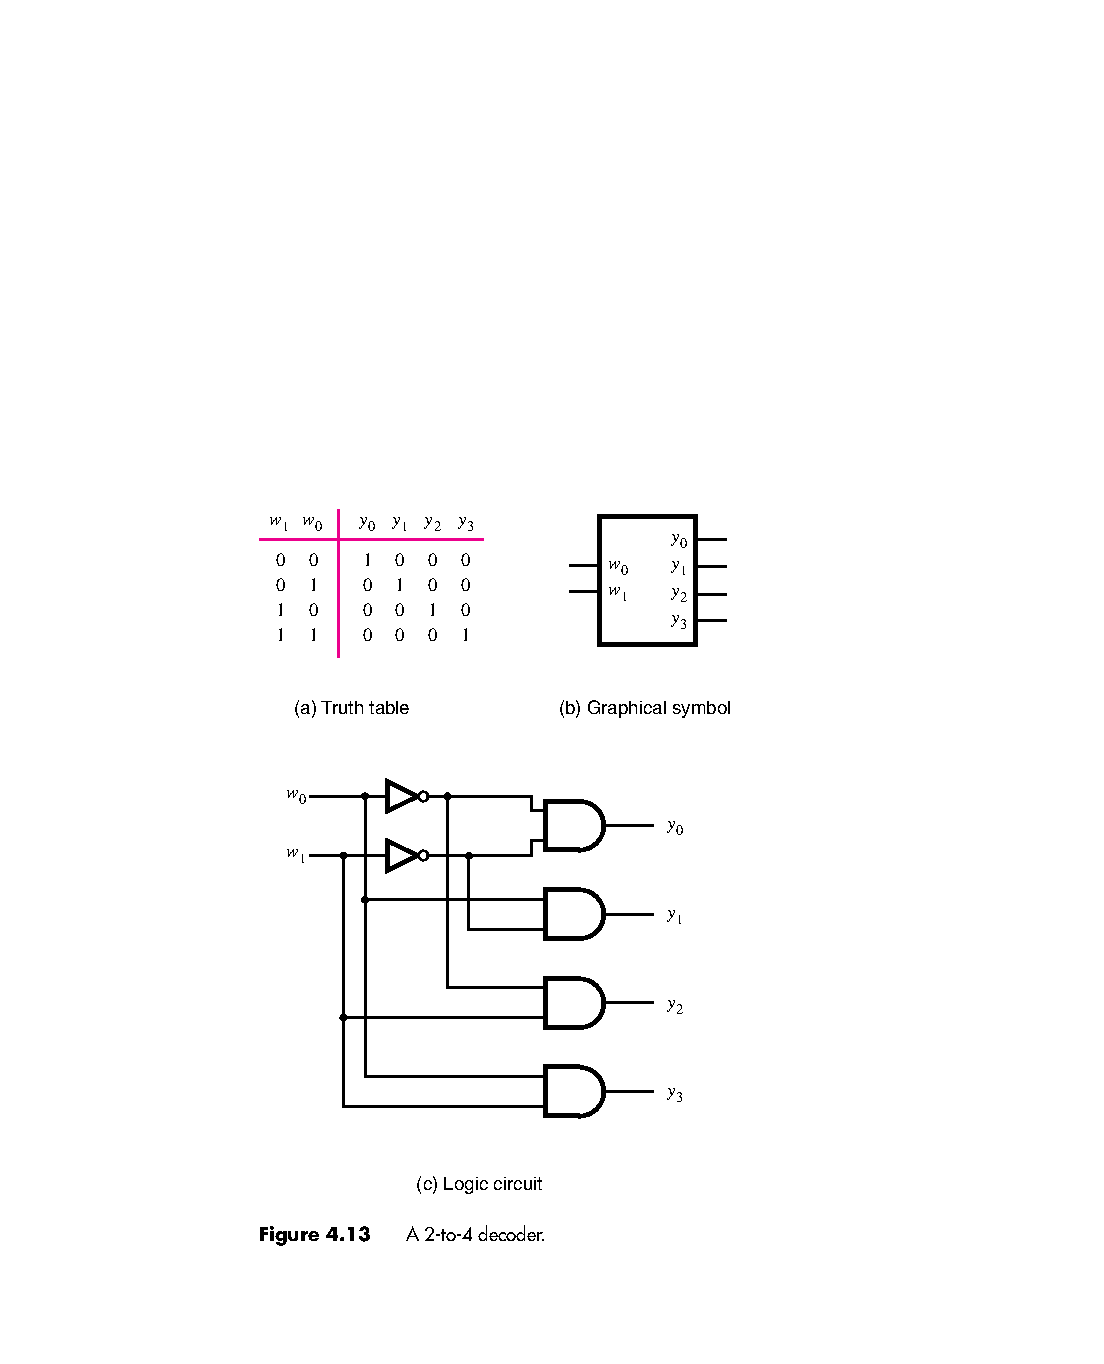
\includegraphics[scale=.85,trim={0 9cm 4cm 0},clip]{VerilogFig4_13} \\
        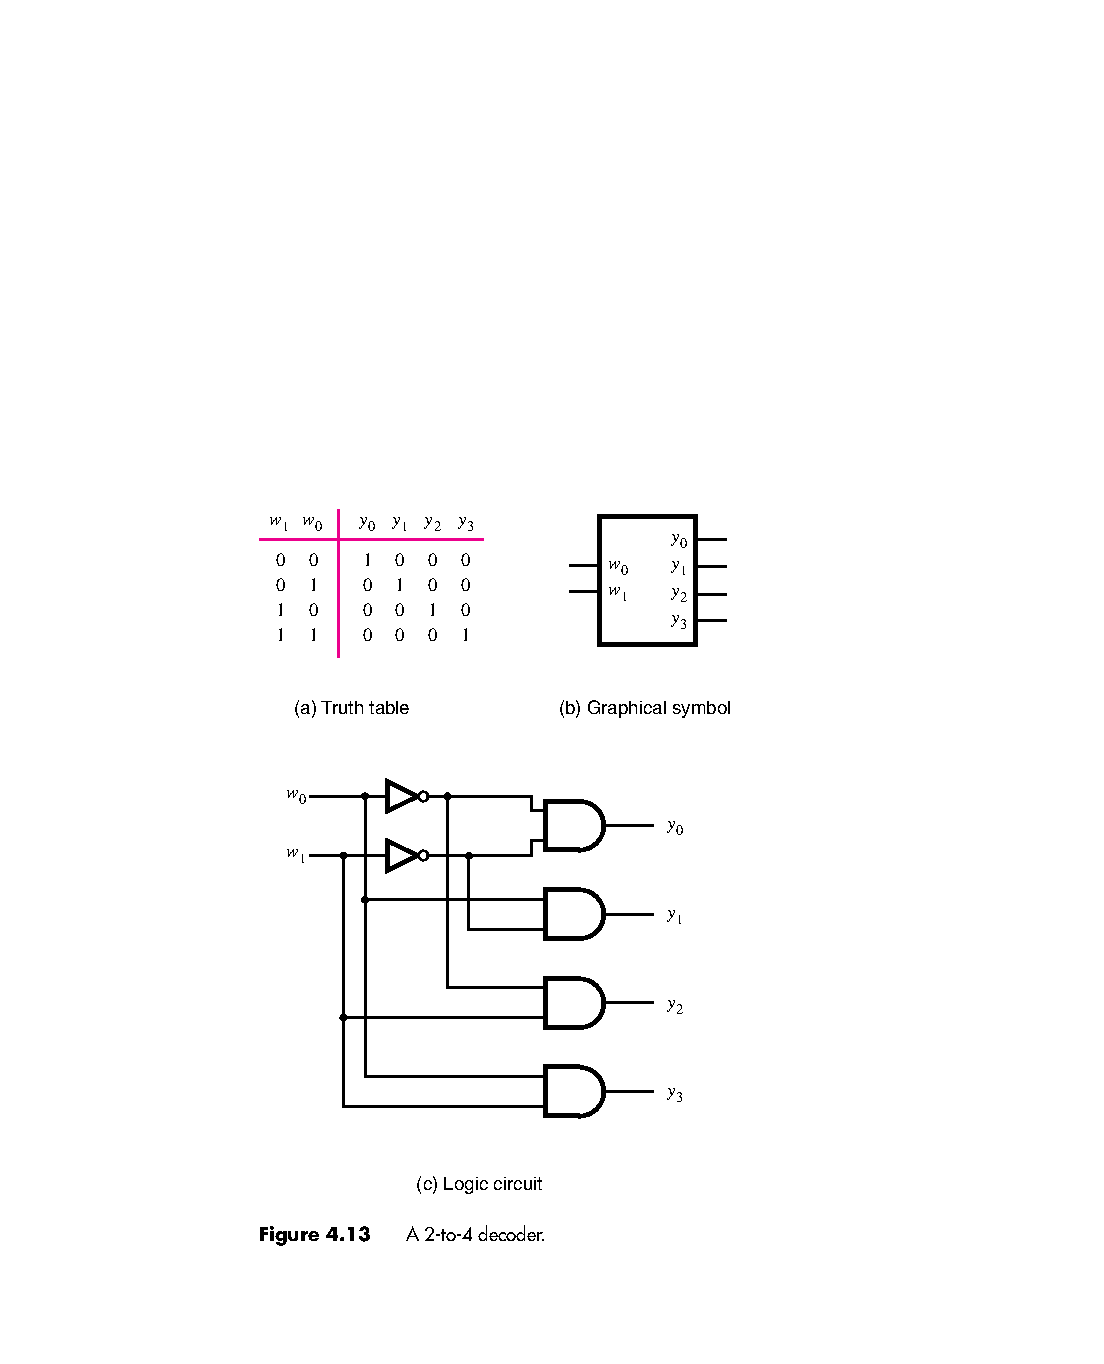
\includegraphics[scale=.85,trim={4.5cm 9cm 0 0},clip]{VerilogFig4_13}
        \end{column}
        \begin{column}{0.60\textwidth}
        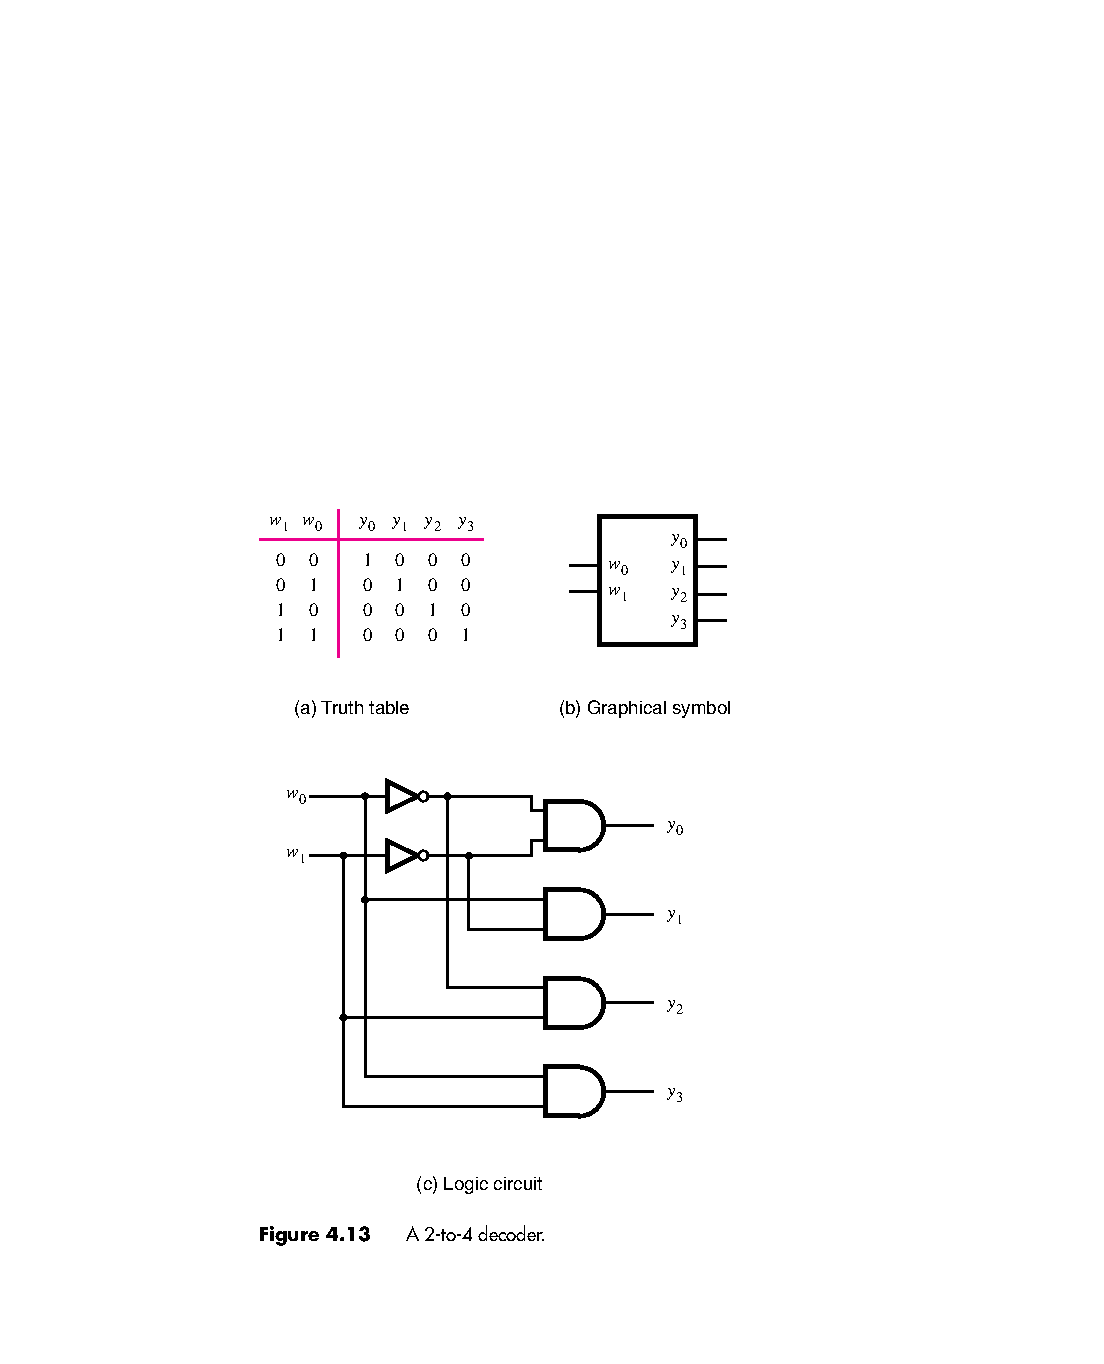
\includegraphics[scale=.85,trim={0 1cm 0 4cm},clip]{VerilogFig4_13}
        \end{column}    
    \end{columns}
    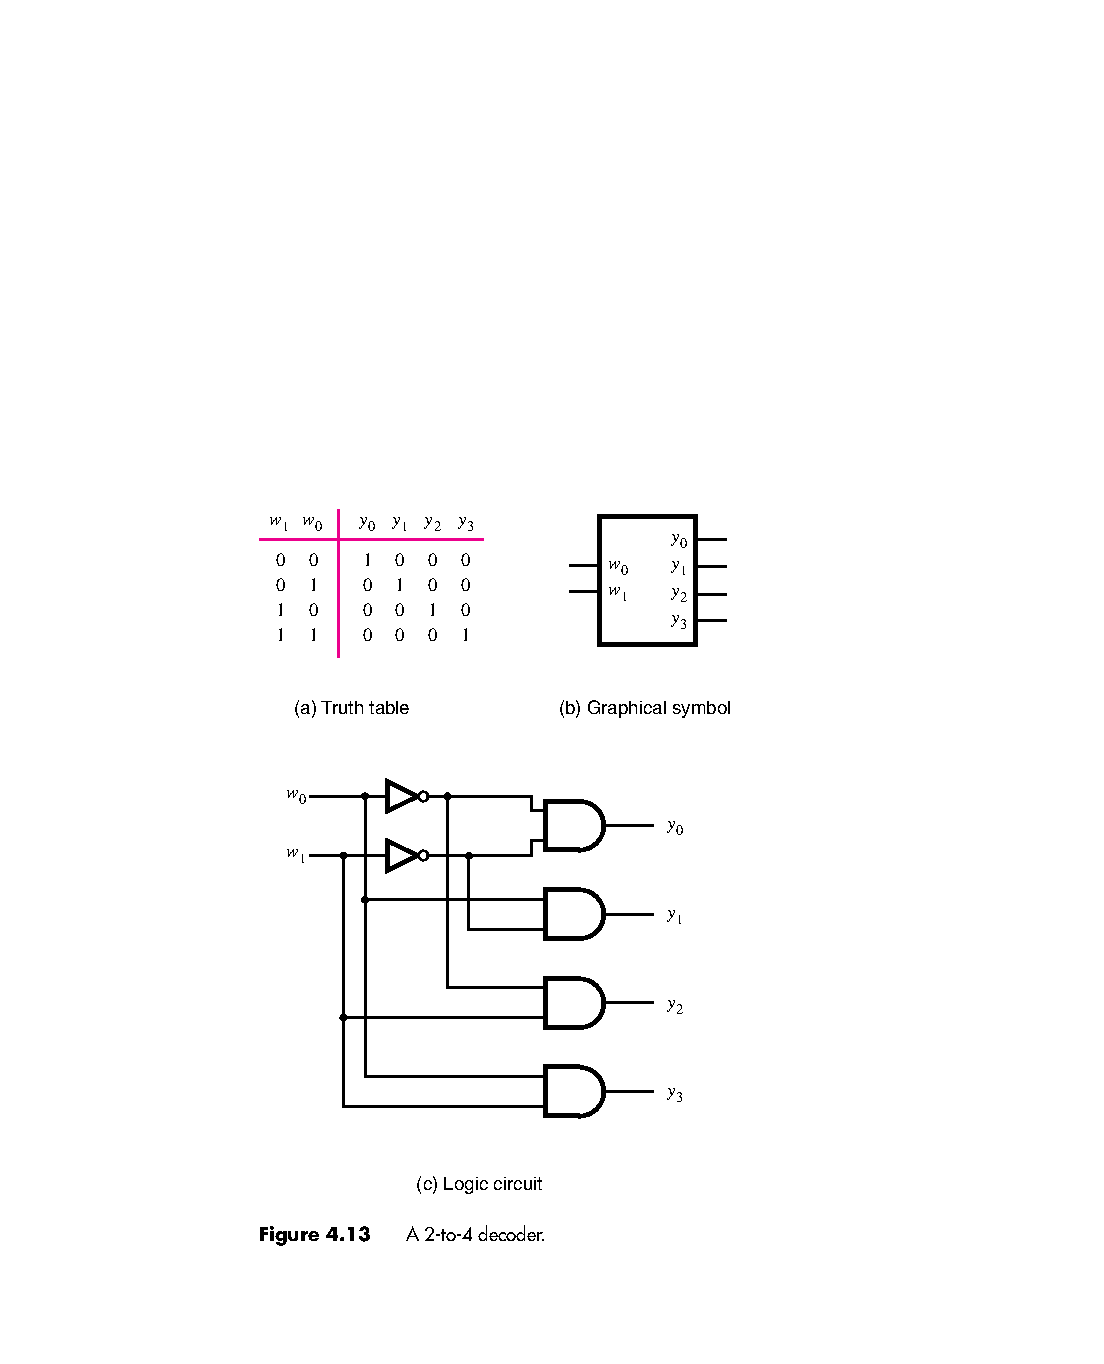
\includegraphics[scale=.85,trim={0 0 3cm 12cm},clip]{VerilogFig4_13}
\end{frame}

\begin{frame}{\insertsection} \centering
    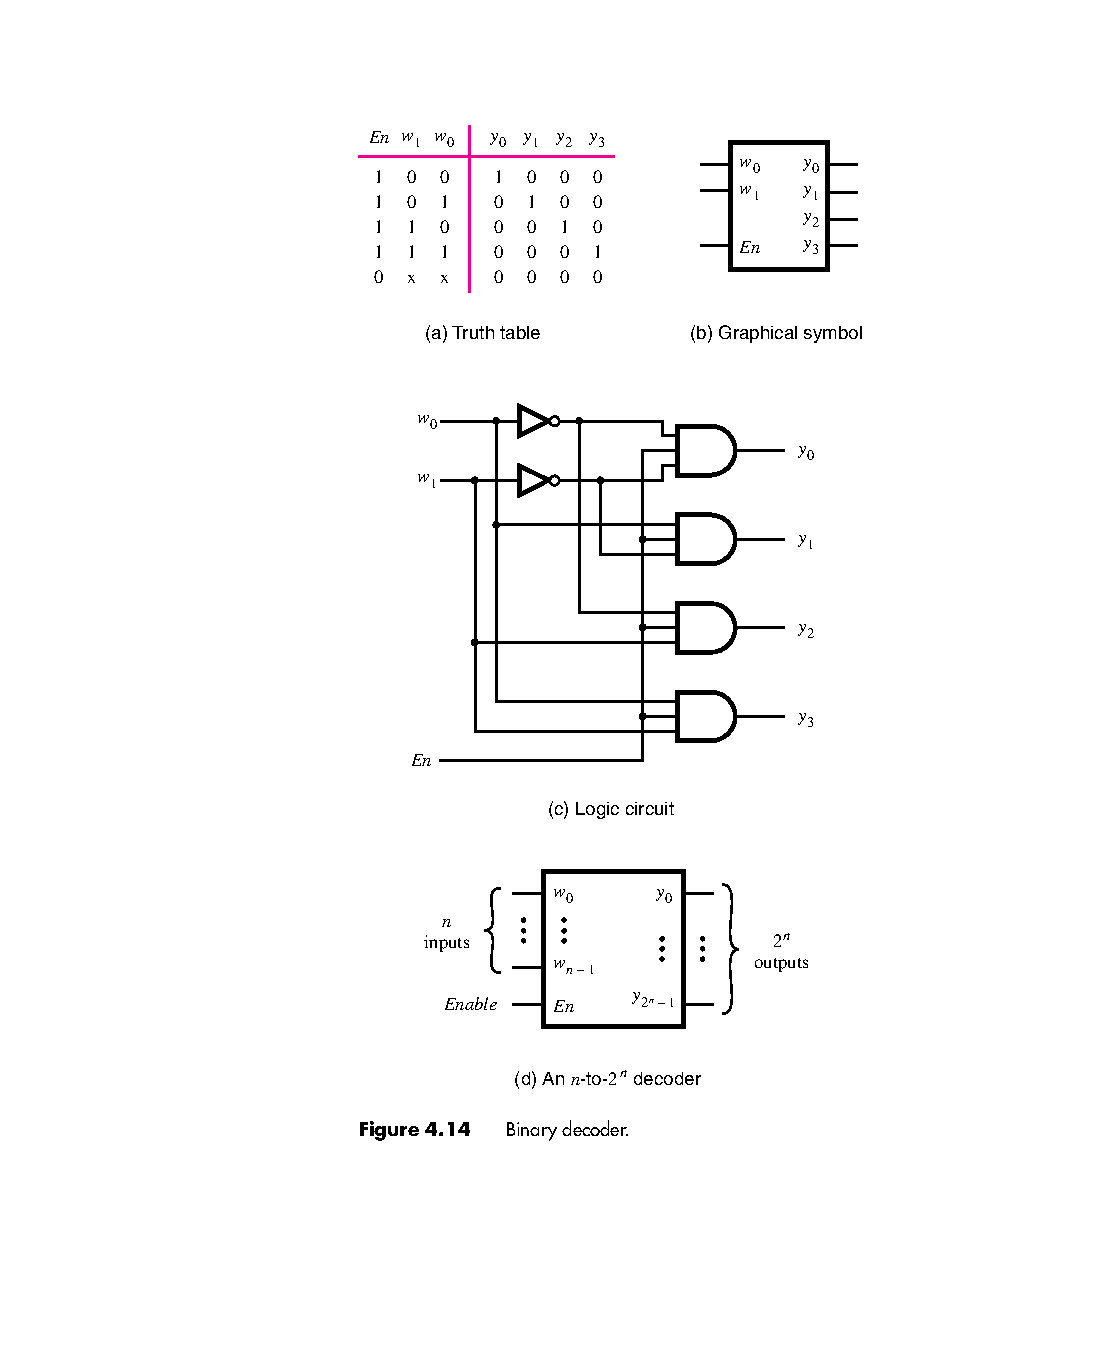
\includegraphics[width=.45\textwidth]{VerilogFig4_14}
\end{frame}

\begin{frame}[fragile]{figure4.31.v}
    \verilog{figure4.31}
\end{frame} 

\begin{frame}[fragile]{figure4.32.v}
    \verilogf{figure4.32}{\scriptsize}
\end{frame} 

\begin{frame}[fragile]{figure4.37.v}
    \verilog{figure4.37}
\end{frame} 

\begin{frame}{\insertsection} \centering
    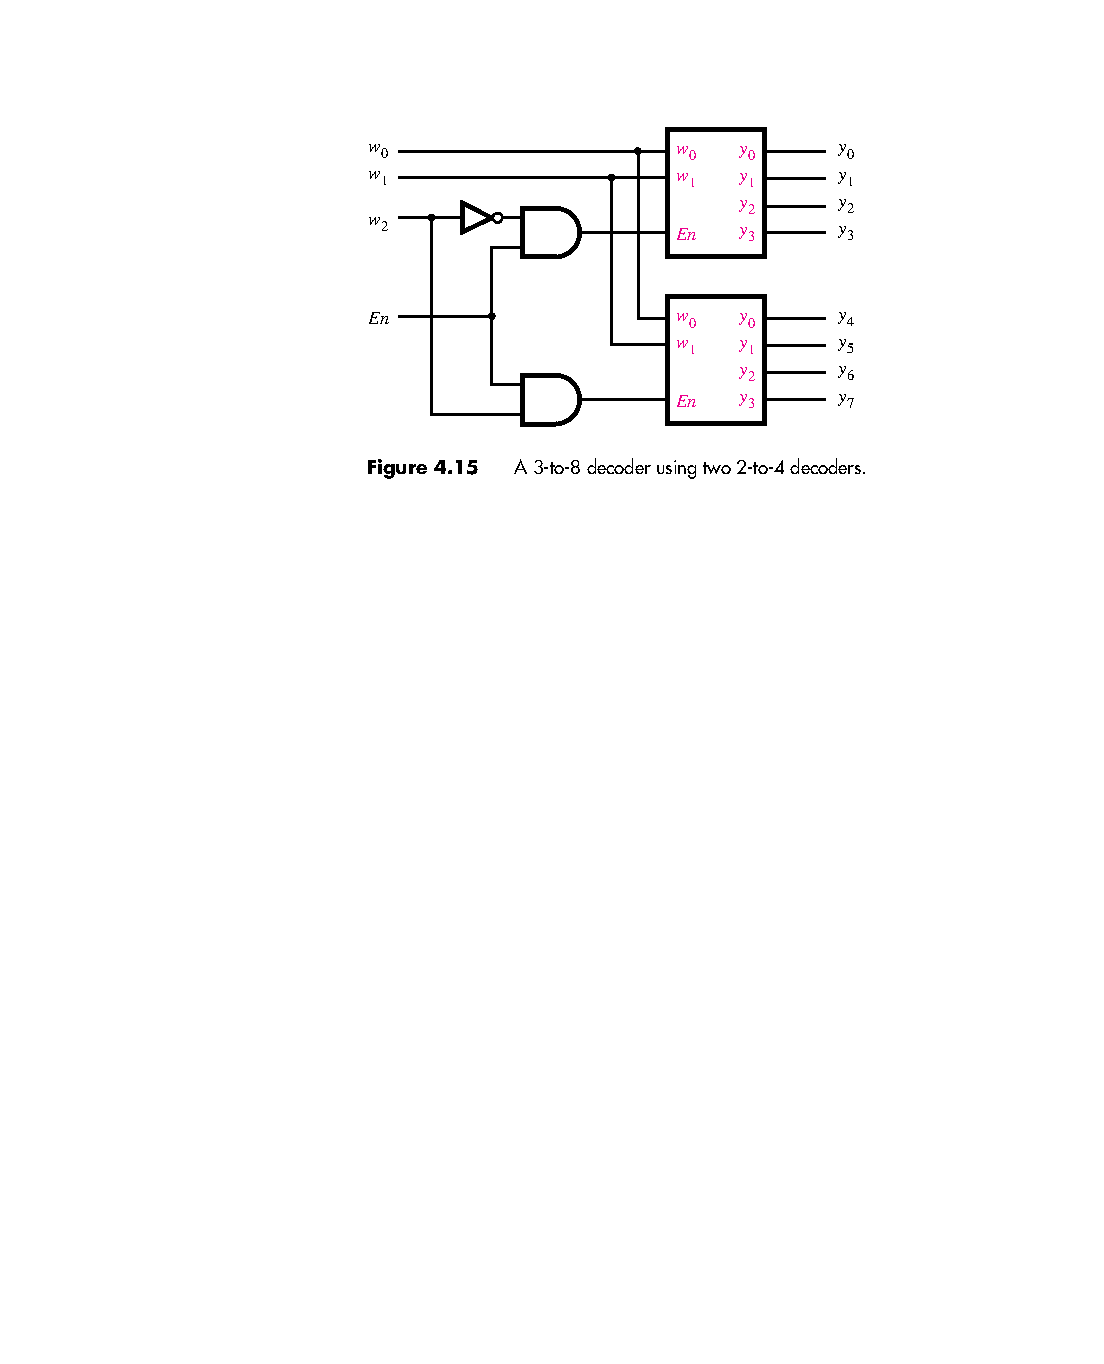
\includegraphics[width=.6\textwidth]{VerilogFig4_15}
\end{frame}

\begin{frame}{\insertsection} \centering
    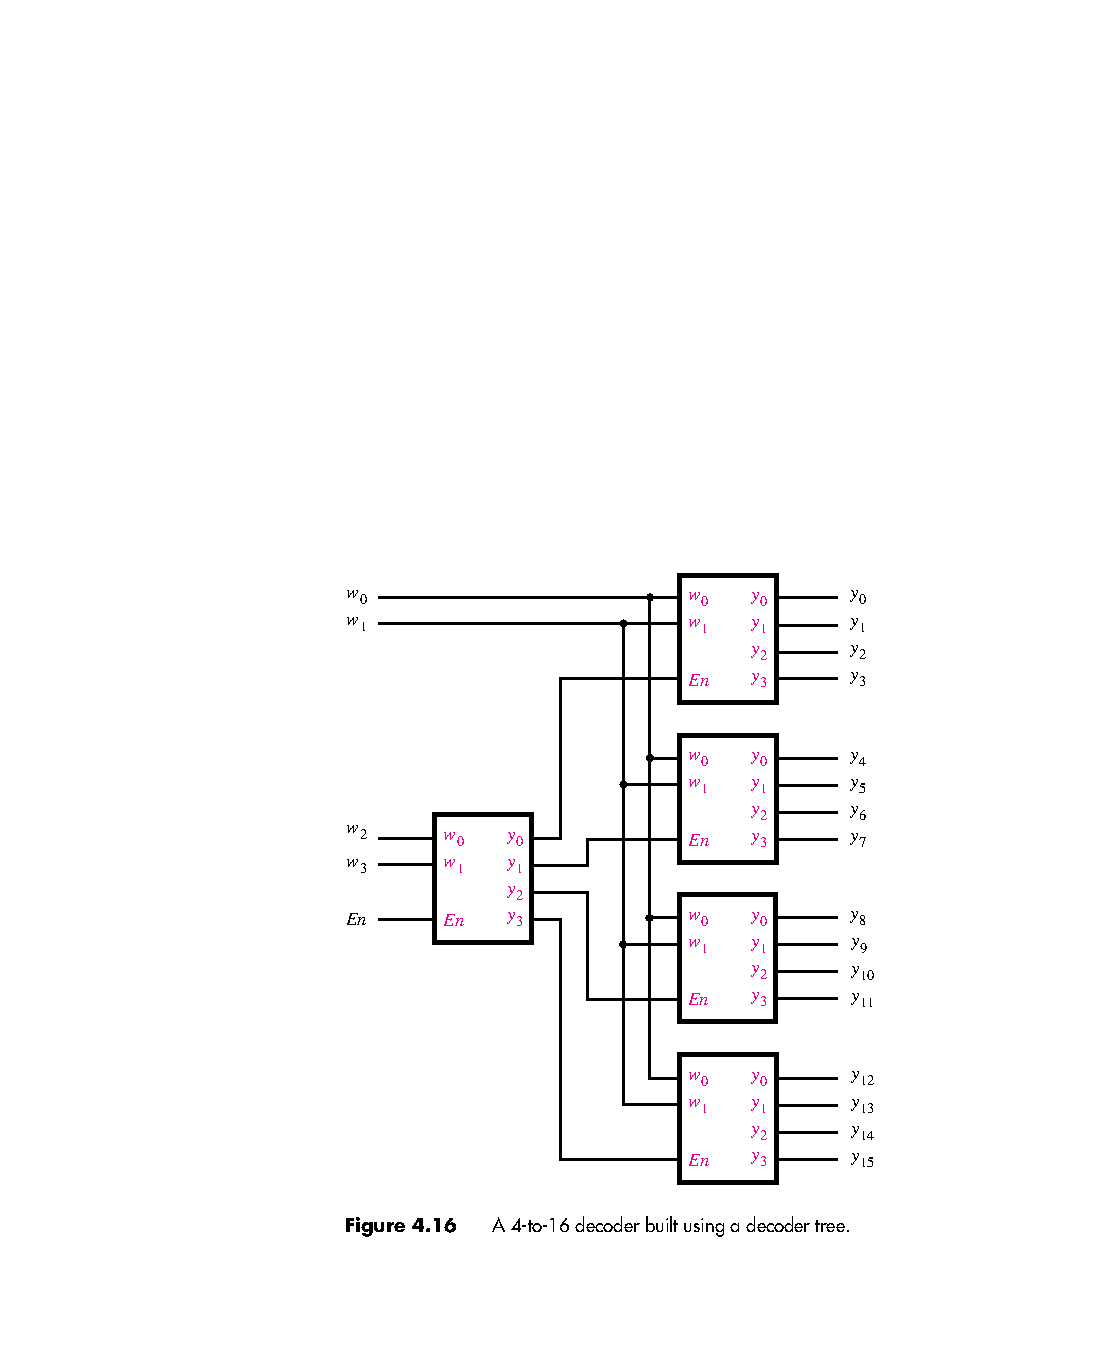
\includegraphics[width=.45\textwidth]{VerilogFig4_16}
\end{frame}

\begin{frame}[fragile]{figure4.33.v}
    \verilog{figure4.33}
\end{frame} 

\begin{frame}{\insertsection} \centering
    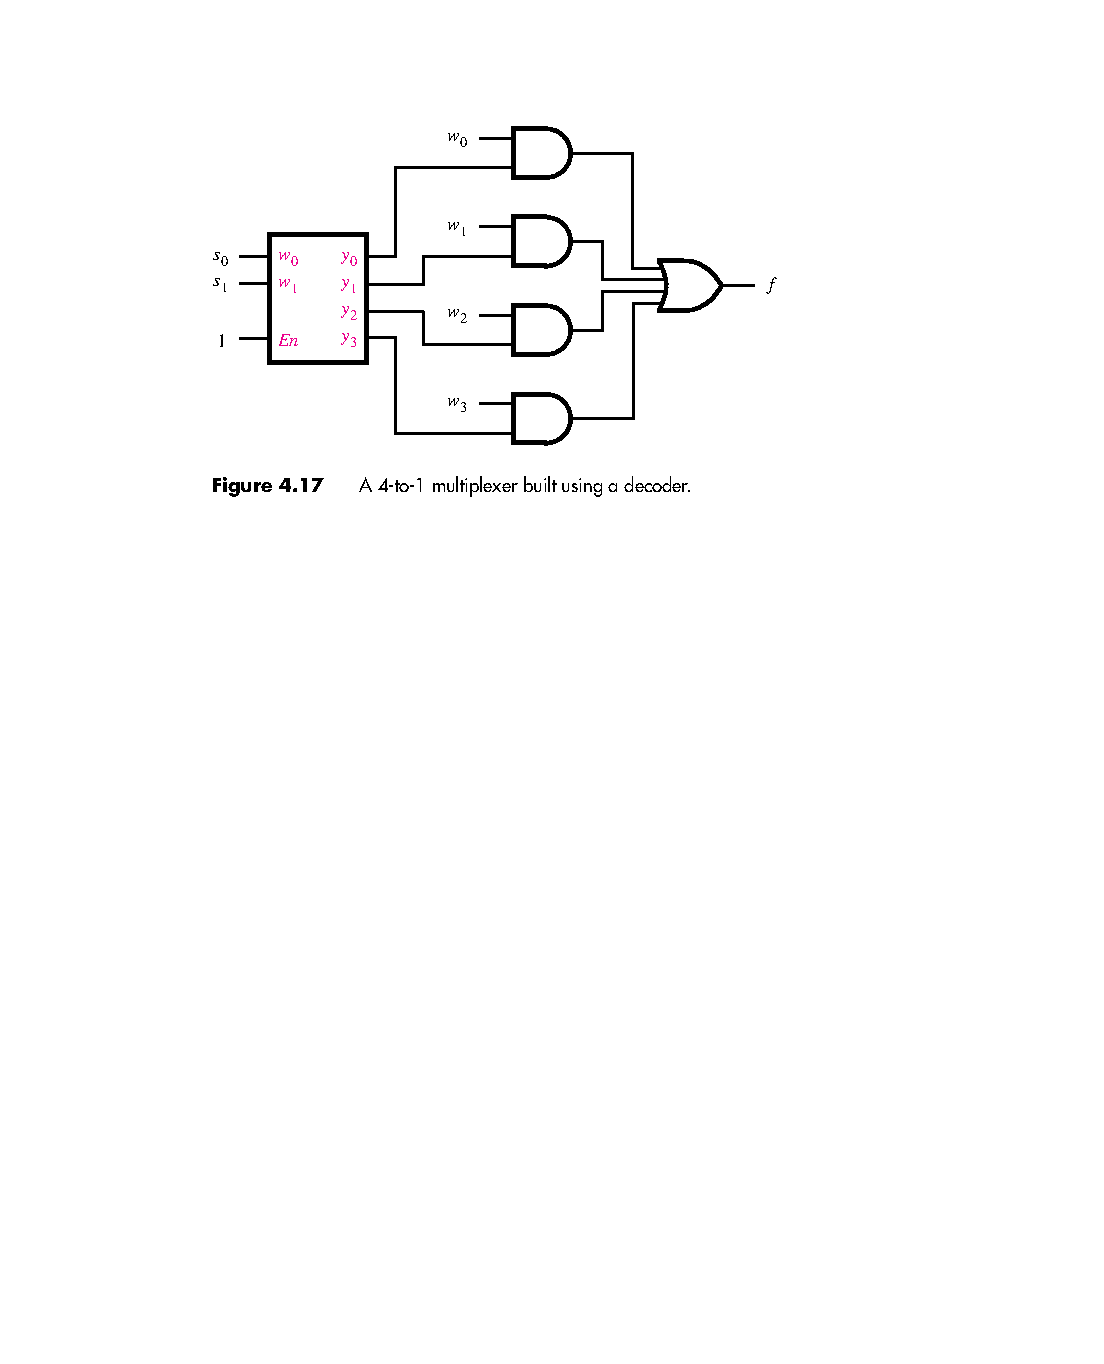
\includegraphics[width=.75\textwidth]{VerilogFig4_17}
\end{frame}

\begin{frame}{\insertsection} \centering
    $f(w_1,w_2,w_3)=\sum m(0,1,3,4,6,7)$ \\
    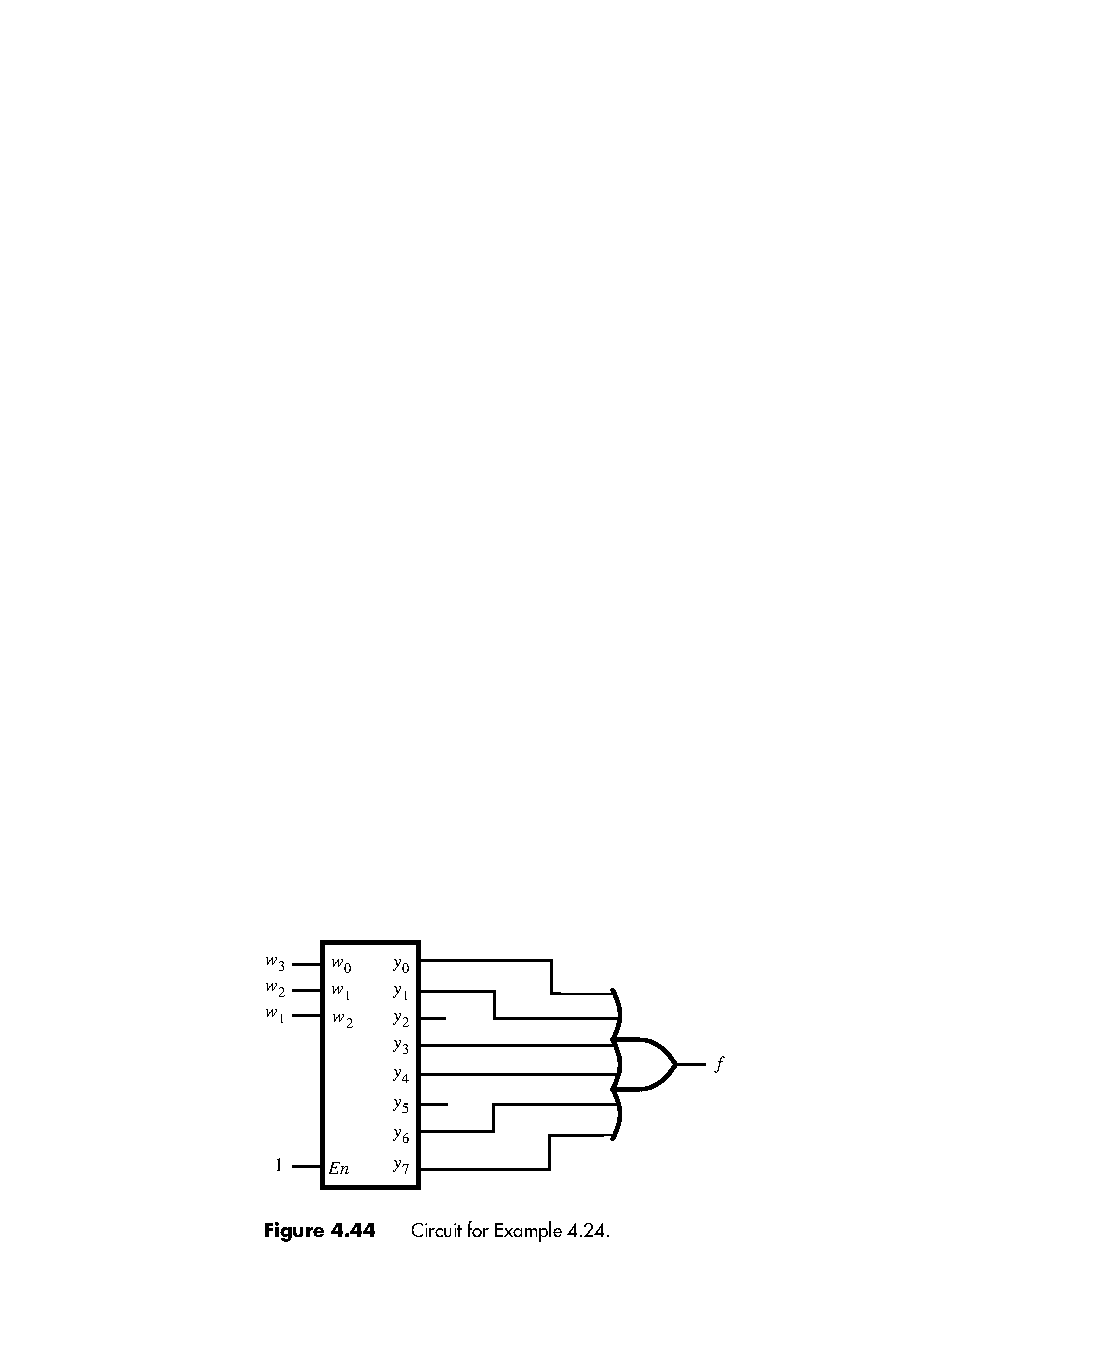
\includegraphics[width=.75\textwidth]{VerilogFig4_44}
\end{frame}

\section{Codificadores}

\begin{frame}{\insertsection} \centering
    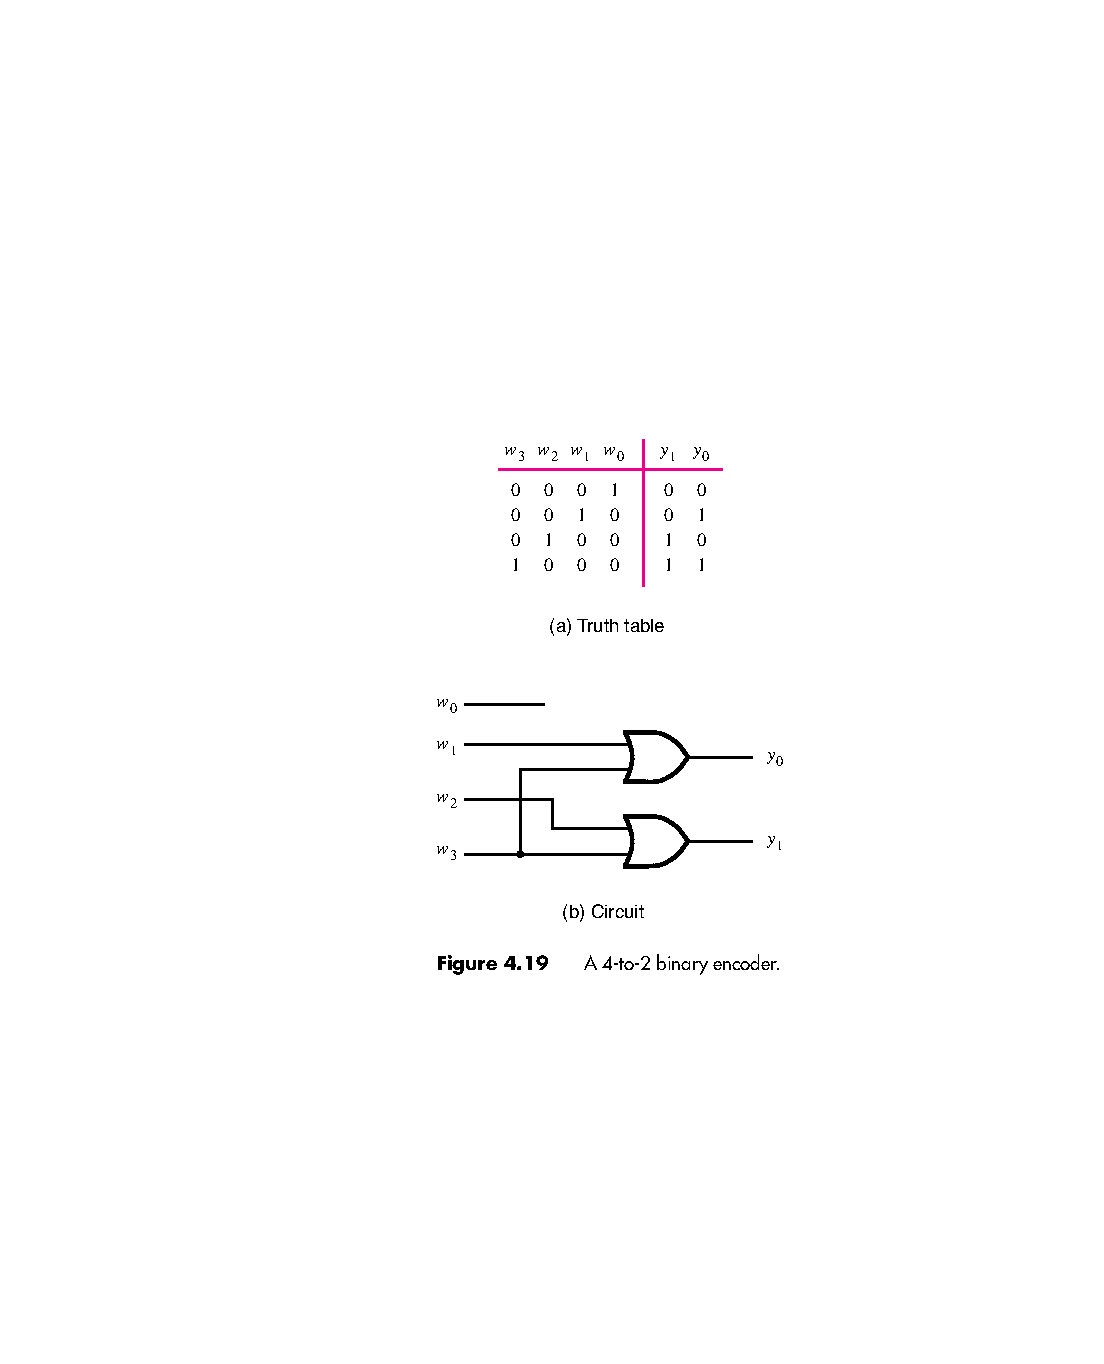
\includegraphics[width=.35\textwidth]{VerilogFig4_19}
\end{frame}

\begin{frame}{\insertsection} \centering
    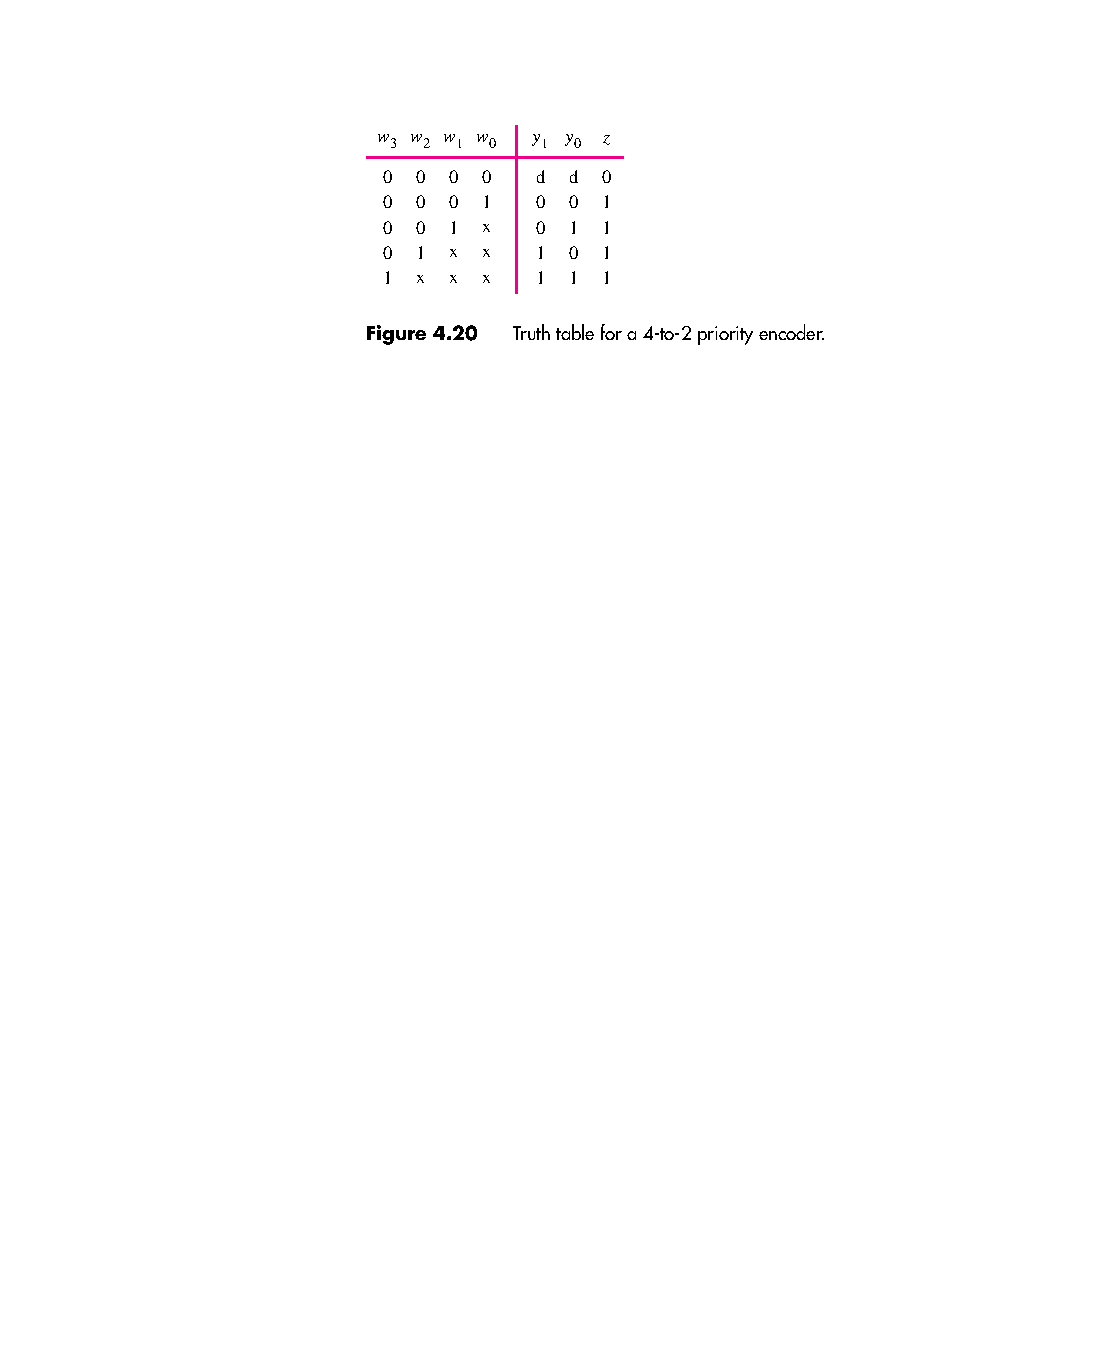
\includegraphics[width=.75\textwidth]{VerilogFig4_20}
\end{frame}

\begin{frame}[fragile]{figure4.36.v}
    \verilogf{figure4.36}{\tiny}
\end{frame} 

\begin{frame}[fragile]{figure4.38.v}
    \verilogf{figure4.38}{\scriptsize}
\end{frame} 

\section{Conversores de Códigos}

\begin{frame}{\insertsection}   \centering
    \begin{columns}
        \begin{column}{0.40\textwidth} \centering
        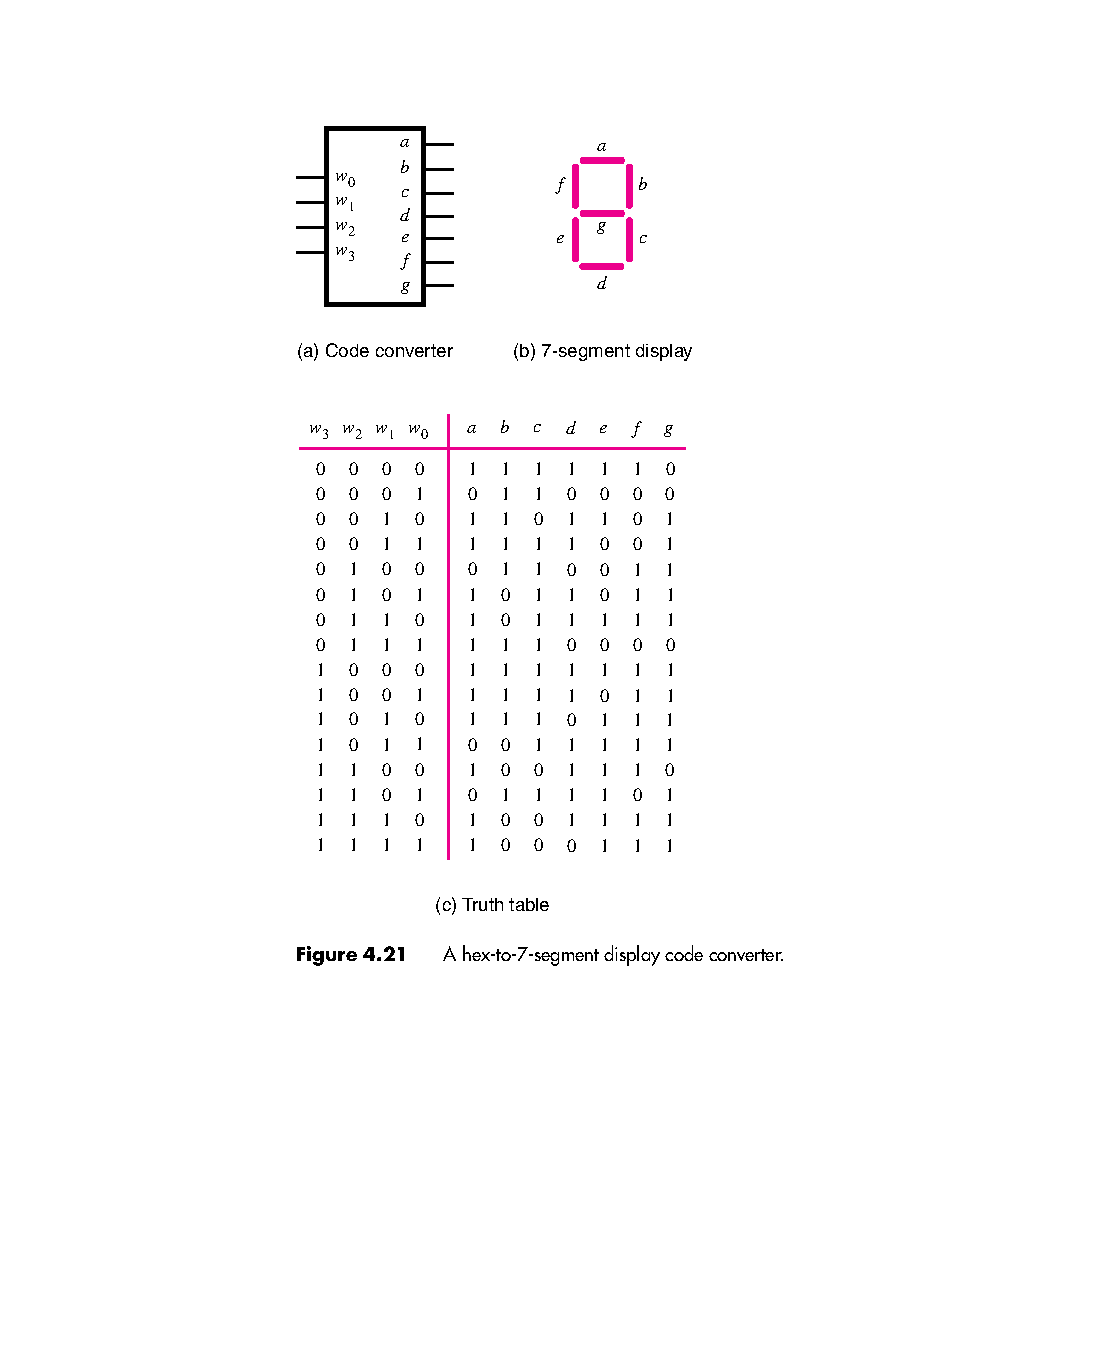
\includegraphics[scale=.75,trim={0 10cm 5cm 0},clip]{VerilogFig4_21} \\
        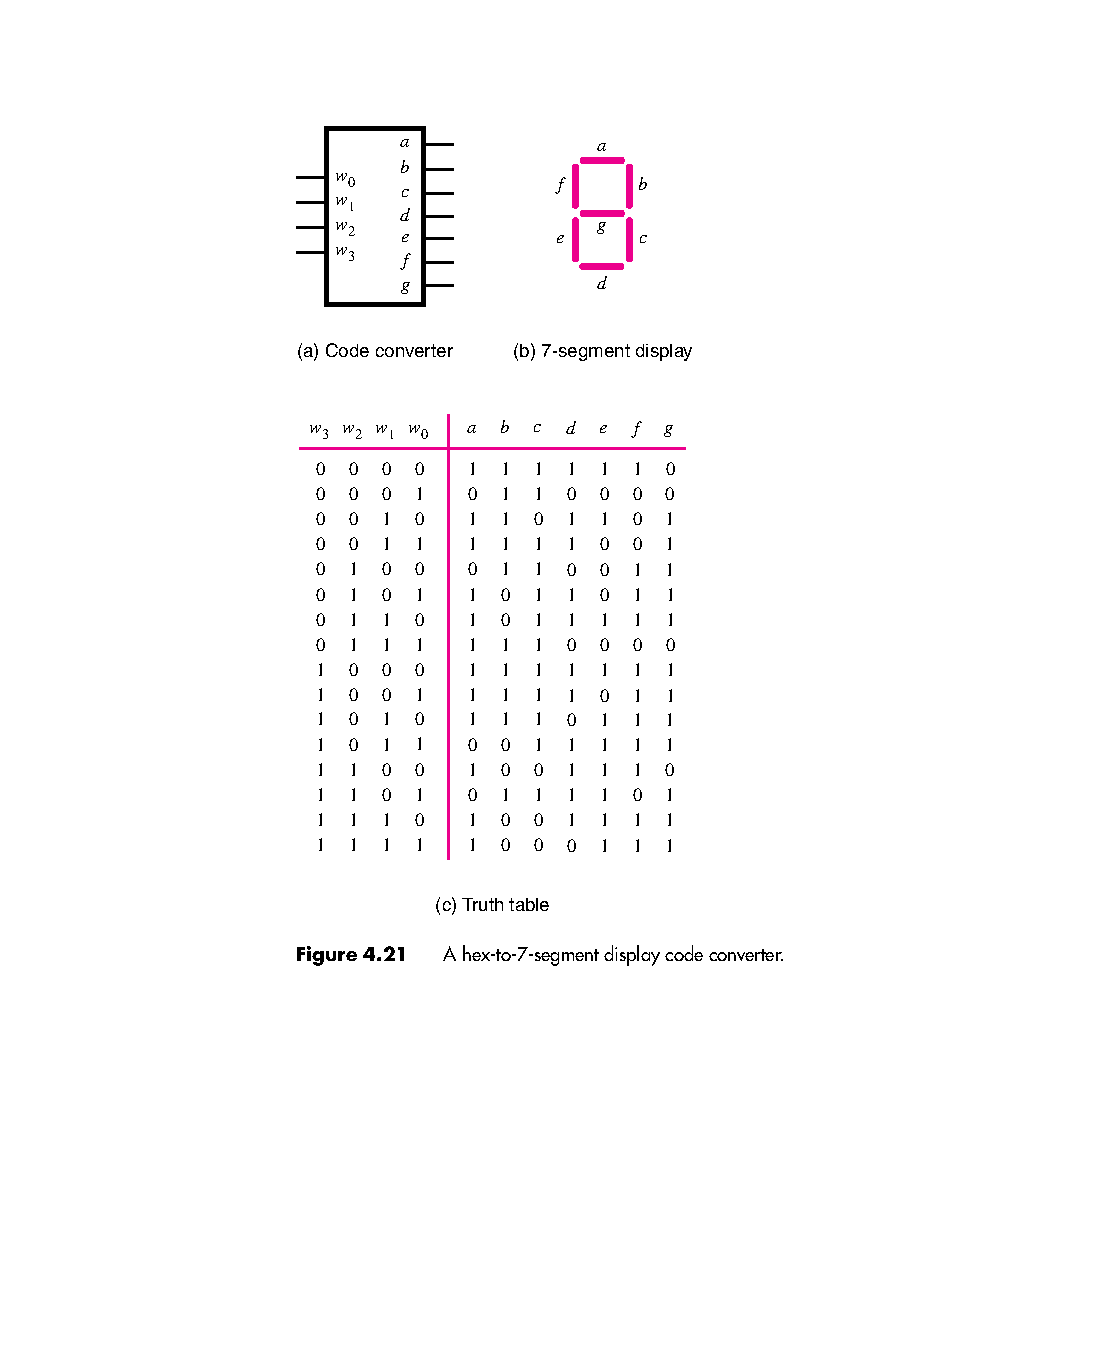
\includegraphics[scale=.75,trim={3.5cm 10cm 1cm 0},clip]{VerilogFig4_21}
        \end{column}
        \begin{column}{0.60\textwidth}
        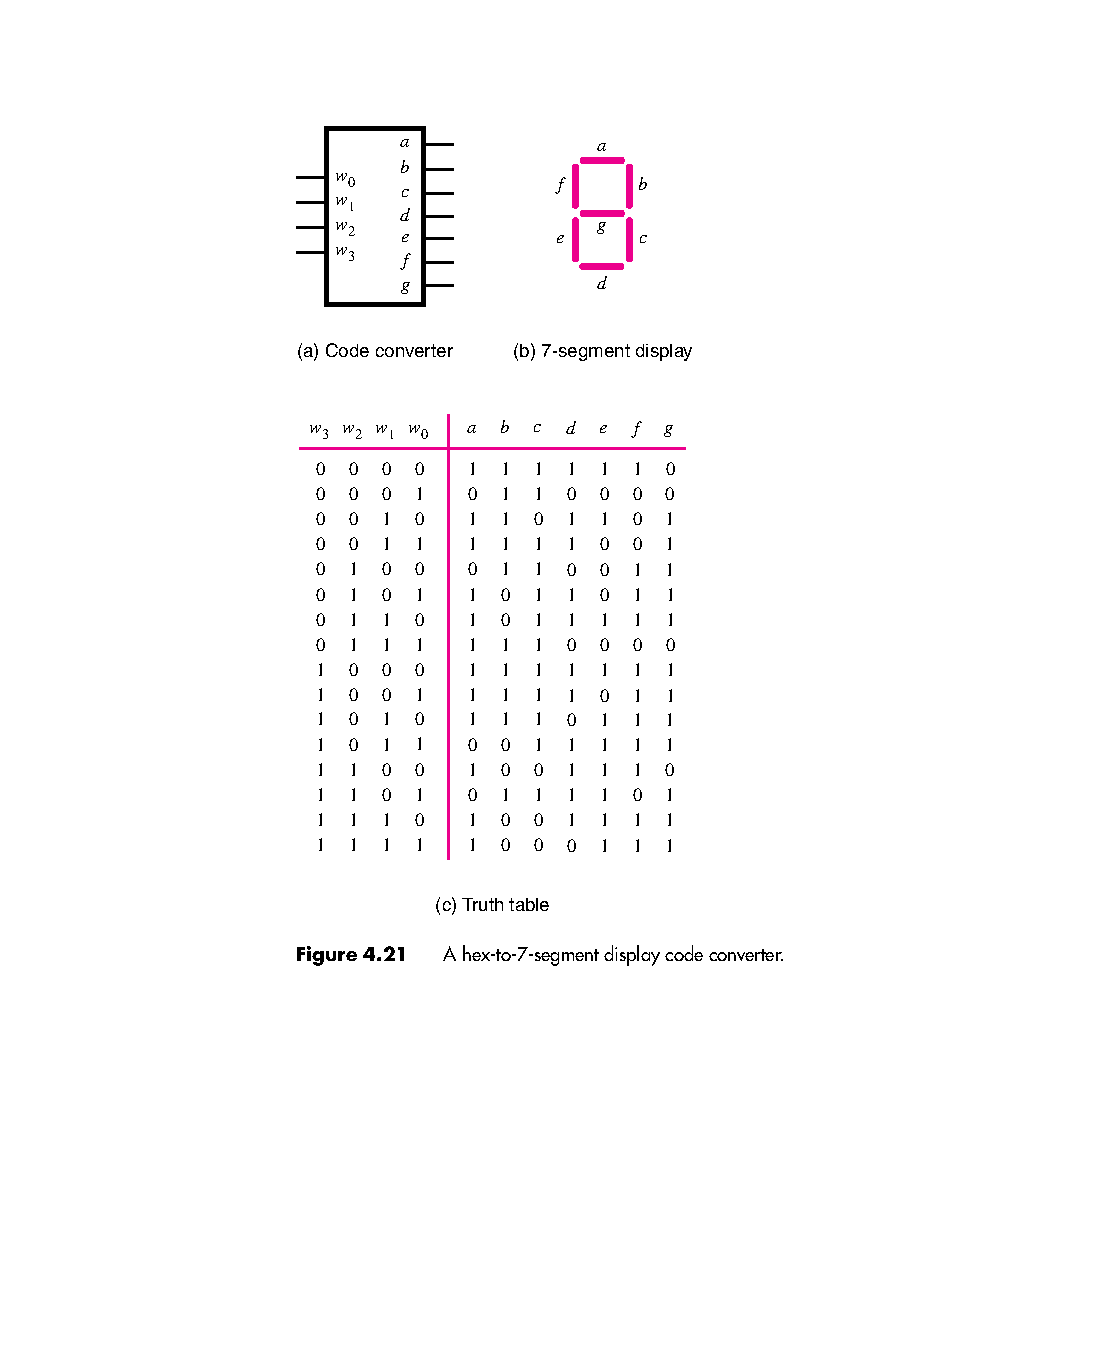
\includegraphics[scale=.75,trim={0 1cm 2cm 5cm},clip]{VerilogFig4_21}
        \end{column}    
    \end{columns}
    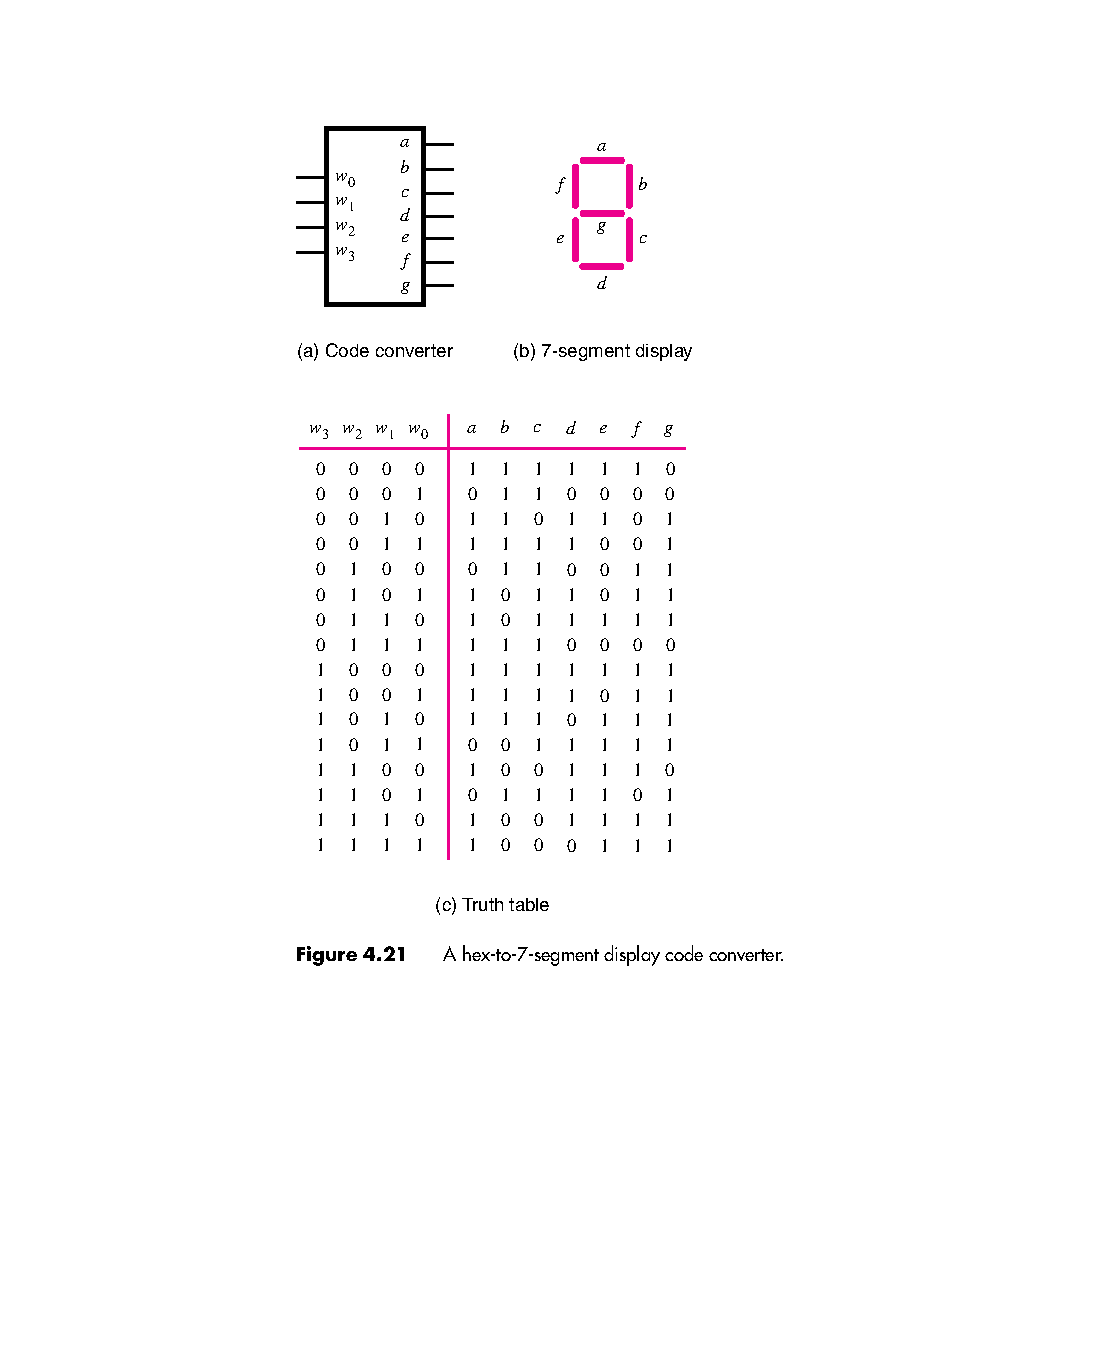
\includegraphics[scale=.75,trim={0 0 0 14cm},clip]{VerilogFig4_21}
\end{frame}

\begin{frame}[fragile]{figure4.34.v}
    \verilogf{figure4.34}{\tiny}
\end{frame} 


\section{Bibliografia} %%%%%%%

\begin{frame}{\insertsection} 
	\begin{itemize}
		\item \href{https://www.google.com.br/search?q=filetype\%3Apdf+Fundamentals+of+Digital+Logic+with+Verilog+Design+&oq=filetype\%3Apdf}{Brown, S. \& Vranesic, Z. - Fundamentals of Digital Logic with Verilog Design, 3rd Ed., Mc Graw Hill, 2009}
	\end{itemize}
\end{frame}

\begin{frame}
	\titlepage
\end{frame} 

\end{document}